\documentclass[12pt]{article}

\usepackage{sbc-template}

\usepackage{graphicx,url}

%\usepackage[brazil]{babel}   
\usepackage[utf8]{inputenc}  
     
\sloppy

\title{Banco de dados em tempo real: Firebase}

\author{Fábio da Silva Takaki\inst{1}, Lucas Martins Valladares Ribeiro\inst{1} }


\address{Faculdade de Ciências e Tecnologia\\
  Universidade Estadual Paulista \\
  "Júlio de Mesquita Filho" \\
  Caixa Postal 19060-900  -- Presidente Prudente -- SP -- Brasil
  \email{fabio@takaki.me, lucasmbtos@live.com}
}

\begin{document} 

\maketitle

\begin{abstract}
   With the emergence of the digital society and the Internet of Things, several concepts for data storage and manipulation have emerged with the purpose of reducing resource and maintenance costs of which Cloud Computing stands out. This article proposes a case study of a tool that addresses one of the service models of the Cloud Computing (IaaS, PaaS and SaaS) architecture, which is Firebase, a tool created by Google. Firebase is a mobile platform that provides a number of services for the rapid development of high-quality web and mobile applications, from which stand out the real-time database service that will be the focus of this work.
\end{abstract}
     
\begin{resumo} 
   Com o surgimento da sociedade digital e a Internet das Coisas, diversos conceitos para armazenamento e manipulação dos dados surgiram com a finalidade de diminiuir os custos de recursos e manutenção do qual destaca-se o Cloud Computing. Este artigo propõe um estudo de caso de uma ferramenta que aborda um dos modelos de serviço da arquitetura Cloud Computing (IaaS, PaaS e SaaS) que é o Firebase, uma ferramenta criada pela Google. O Firebase é uma plataforma mobile que fornece diversos serviços para o rápido desenvolvimento de aplicativos web e móveis de alta qualidade, do qual destaca-se o serviço de banco de dados em tempo real que será o foco principal deste trabalho.
\end{resumo}


\section{Introdução}

%  descrição do cenário e problemas em aberto
A popularização da internet gerou uma sociedade digital, o que antigamente era local, tornou-se online. O volume de informações se propagou de forma abundante nos últimos anos, principalmente com o avanço das tecnologias móveis. Em decorrência disso, diversos conceitos para armazenamento e manipulação dos dados surgiram com a finalidade de diminuir os custos de recursos e manutenção. Com efeito, originaram-se recursos como \cite{WA} \cite{GAE} \cite{AWS}, os quais seguem conceitos de um modelo novo, o \textit{Cloud Computing}. Até então, não existiam serviços que supriam as necessidades essenciais de voltadas para aplicativos atuais (chats e redes sociais), que demandam desenvolvimento móvel/web com armazenamento e sincronização de dados em tempo real. O presente artigo descreve um estudo de caso do \textit{Firebase}, que tem por finalidade fornecer um serviço de dados em nuvem em tempo real, utilizado para criação de aplicativos multiplataformas que compartilham um banco de dados não relacional que a própria ferramenta disponibiliza, do qual será o foco principal deste trabalho. Como consequência, a ferramenta possibilita aos desenvolvedores criarem aplicativos de alta qualidade de forma rápida e fácil, sem a necessidade de se preocupar com infraestrutura e escalabilidade de recursos.
\\
Este artigo está organizado da seguinte maneira: na Seção II será apresentado uma fundamentação teórica sobre \textit{Cloud Computing}, em que é essencial para o entendimento do Firebase; na Seção III será apresentado a metodologia de apoio; na Seção IV um estudo de caso da ferramenta firebase em que é realizado um estudo do desenvolvimento de uma aplicação; por fim na Seção V, resultados e trabalhos futuros.

\section{\textit{Cloud Computing}} \label{sec:firstpage}

\textit{Cloud computing} é uma tecnologia em que os recursos de \textit{hardware} e \textit{software}, tais como aplicações especiais, CPU, armazenamento e muitos outros são fornecidos aos usuários através da Internet como um serviço, e é cobrado com base no que você usa \cite{1}. Como os recursos são fornecidos através da Internet, o usuário não se preocupa com a manutenção e suporte deles. Esses recursos têm a capacidade de escalabilidade automática de acordo com a demanda do cliente. 

O conceito de \textit{Cloud Computing} é classificado em três modelos de serviço: \textit{Software as a Service} (SaaS), \textit{Plataform as a Service} (PaaS) e \textit{Infrastructure as a Service} (IaaS). Com isso, é possível criar uma representação dos modelos de serviço por meio de camadas de virtualização (Figura~\ref{fig:architeture}).

\begin{figure}[ht]
\centering
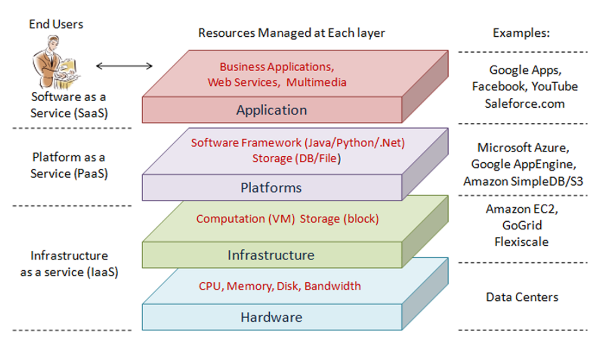
\includegraphics[width=.9\textwidth]{architeture.png}
\caption{Arquitetura \textit{Cloud Computing} (retirado de: \cite{2})}
\label{fig:architeture}
\end{figure}

\textbf{\textit{Infrastructure as a Service}}

O serviço oferece, como o próprio nome já diz, a infraestrutura. Compondo a base das camadas de virtualização, é responsável pelo \textit{hardware}.
Ao invés de manter hacks, servidores e roteadores, o usuário contrata sevidores virtuais, que armazenarão de forma comum á aqueles. Os tipos de cobrança mais comuns são: número de servidores e o tráfego de dados utilizado.

\textbf{\textit{Platform as a Service}}

Plataforma como serviço, tradução literal, é o serviço entre \textit{Infrastructure as a Service} e \textit{Software as a Service}. É proporcionar um ambiente ou plataforma apropriada na qual o desenvolvedor pode criar as aplicações e o \textit{software}, através da Internet, sem necessidade de instalação ou gerenciar o ambiente de desenvolvimento \cite{1}. O serviço fornece ao usuário um ambiente flexível e adequado que suporta as tecnologias que deseja, como frameworks ou linguagens de programação. Como observado na figura~\ref{fig:architeture}, temos o modelo de serviço \textit{Google App Engine}, o qual oferece uma plataforma de desenvolvimento para aplicações web e móvel.

\textbf{Software as a Service}

Entrando na última camada de serviços, observamos o \textit{Software as a Service}. Esse modelo propõe um software como serviço fornecido através da internet, não necessitando de sua instalação. O fornecedor deste modelo de serviço é responsável por controlar e limitar o uso das aplicações. Portanto, o cliente deste modelo de serviço também fica livre da necessidade de uma infraestrutura, já disponibilizada pelo fornecedor.

Assim, com os conceitos de \textit{Cloud Computing}, o \textit{Firebase} é considerado \textit{Platform as a Service}, por ser uma plataforma de desenvolvimento que oferece armazenamento e sincronização de dados em tempo real, utilizando apenas código \textit{client-side}. 

\section{Metodologia de Apoio ao \textit{Firebase}}  \label{sec:metodologia}

\textit{Firebase} foi criado em 2011 por Andrew Lee e James Tamplin porém foi lançado oficialmente em 2012. Originalmente, o sistema tinha o intuito de fornecer um banco de dados em tempo real, fornecendo uma API aos usuários para armazenar e sincronizar dados através de diferentes clientes \cite{3}. Assim, a metodologia do \textit{Firebase} mudou um pouco após a aquisição da Google. Dois anos depois de sua \textit{release}, surgiram diversos serviços que complementam a ideia do banco de dados em tempo real, voltados para aplicativos móveis ou web: \textit{Firebase Auth}, \textit{Firebase Storage}, \textit{Firebase Cloud Messaging}, \textit{Firebase Remote Config}, \textit{Firebase Test Lab for Android} e \textit{Firebase Crash Reporting}. Dentre todos os serviços citados nesta seção, este trabalho foca no objetivo inicial do \textit{Firebase} que é o \textit{real-time database}.

\subsection{Acesso e criação de projetos}

O acesso à todos os serviços (citados na Seção \ref{sec:metodologia}) do \textit{Firebase}, é preciso apenas de uma conta Google, que pode ser criada gratuitamente. Concedido o acesso ao console do \textit{Firebase}, facilmente você cria um projeto apenas especificando o nome do projeto, e assim é liberado o acesso à todos os serviços. Para o uso da API, necessita apenas do desenvolvedor configurar a aplicação web ou mobile desejada com as \textit{keys} da API do \textit{Firebase} que é fornecida logo após a criação de um projeto, carregando a biblioteca \textit{firebase}.

\subsection{\textit{Firebase Realtime Database}}

O \textit{Firebase Realtime Database} é um banco de dados hospedado em nuvem. Os dados são armazenados como JSON e sincronizados em tempo real para cada cliente conectado. Ao criar aplicativos multiplataforma com nossos SDKs para iOS, Android e JavaScript, todos os seus clientes compartilham uma instância do \textit{Realtime Database} e recebem automaticamente atualizações com os dados mais recentes \cite{Firebase}. Portanto, o objetivo do \textit{Firebase Realtime Database} é fornecer um banco de dados em tempo real, em que o cliente é conectado diretamente e só é preciso enviar os dados através de uma API.

\textbf{Como os dados são armazenados}

Todos os dados são armazenados na nuvem do \textit{Firebase} em objetos JSON formando uma árvore. Quando um dado é adicionado no banco de dados, o dado se torna em um nó na árvore JSON do qual o \textit{Firebase} associa uma chave à esse nó para manipulações futuras. Nesse sentido, um exemplo de um chat em que o usuário tem seu próprio perfil com sua lista de contatos, a árvore JSON se tornaria algo como na Figura~\ref{fig:json-tree}.

\begin{figure}[ht]
\centering
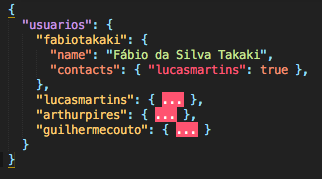
\includegraphics[width=.5\textwidth]{json-tree.png}
\caption{Exemplo de uma estrutura JSON de uma aplicação chat.}
\label{fig:json-tree}
\end{figure}


\textbf{Segurança e Regras}

O \textit{Firebase Realtime Database} tem uma área (\textit{Firebase Realtime Database Rules}) onde há configurações e regras que determinam quem tem acesso a leitura e gravação no banco de dados, como os dados estão estruturados e o qual índices existem. Todas as regras ficam armazenadas nessa área do \textit{Firebase} e podem ser alteradas a qualquer momento na ferramenta. Portanto, todas as operações de leitura e gravação só serão concluídas se as regras armazenadas no \textit{Firebase Realtime Database Rules} permitirem. 

A estrutura em que as regras são definidas também são armazenadas em JSON que seguem uma sintaxe e são definidas em quatro tipos: 
\begin{enumerate}
  \item \textbf{\textit{.read}} - Descreve se e quando os dados podem ser lidos pelos usuários.
  \item \textbf{\textit{.write}} - Descreve se e quando os dados podem ser escritos.
  \item \textbf{\textit{.validate}} - Define o aspecto correto de um valor formatado, se ele tem atributos filho e o tipo de dados.
  \item \textbf{\textit{.indexOn}} - Especifica uma criança a indexar para suportar pedidos e consultas.
\end{enumerate}

O \textit{Firebase Realtime Database} é pré-configurado com o \textit{Firebase Auth}, que é responsável por realizar a segurança do app quando sua natureza são dados restritos aos usuários autenticados. Como o intuito deste trabalho é realizar um estudo de caso do serviço de banco de dados em tempo real, foi configurado as permissões de leitura e gravação como público, não necessitando de autenticação para efetuar ambas operações.

\textbf{API do \textit{Firebase}}

A API do \textit{Firebase} é manipulada através de bibliotecas desenvolvidas pela Google em que é facilmente carregada em projetos Android, iOS ou Web. Assim, o \textit{Firebase} conta com uma variedade de métodos em sua biblioteca para a realização de qualquer tipo de operação direta com o banco de dados, com a sua principal característica que são operações em tempo real. 

\subsection{Implementação de um chat com \textit{Firebase}}

Para a realização do estudo de caso para o \textit{Firebase}, foi implementado uma aplicação chat, que são aplicações muito comuns hoje em dia e necessitam de uma sincronização e armazenamento em tempo real. Nesse sentido, foi criado um projeto novo no \textit{Firebase} utilizando a biblioteca Javascript voltado para aplicações web e mobile (híbridas) realizando as operações CRUD de um chat público. Com isso,  demonstraremos como seria a mesma aplicação implementada com bancos de dados tradicionais relacionais ou não relacionais.

\textbf{Enviando Mensagens (\textit{CREATE})}

O envio de mensagens com o \textit{Firebase} pode ser realizado através do método \textit{\textbf{.push(objeto)}} da biblioteca do \textit{Firebase}, em que o objeto com as informações são passadas como parâmetro. No caso do chat utilizamos uma estrutura bastante simples do qual o objeto JSON tem apenas o nome do usuário que está enviando a mensagem e a mensagem em si. Em bancos de dados tradicionais, é preciso instalar o banco de dados e utilizar de uma linguagem \textit{backend} para conexão com o banco de dados para a inserção dos dados no banco. Se caso for um banco de dados relacional, é preciso definir a estrutura da mensagem em uma tabela com os campos de nome de usuário e a mensagem.

\textbf{Recebendo Mensagens (\textit{READ})}

Com o propósito do \textit{Firebase} de realizar o banco de dados em tempo real, o recebimento das mensagens de uma aplicação em chat fica extremamente simples. Com o método \textit{\textbf{.on(evento, callback)}}, a aplicação interage através de eventos passados parâmetro. Assim, com o evento \textit{child\_added} é disparado quando algum novo objeto da referência que está estanciada é adicionado no banco de dados. Então, a função \textit{callback} é chamada, em que é passada no segundo parâmetro do método \textbf{.on()}, tem seu parâmetro que tem um valor do objeto JSON adicionado. Então, é através dessa função de \textit{callback}, é possível atualizar a lista de mensagens com a nova mensagem adicionada no banco à todos os usuários que estiverem com a aplicação de chat aberta. A implementação com bancos de dados tradicionais nessa parte do chat, é preciso implementar um \textit{socket} entre todos os usuários que estão conectados na aplicação, que após a inserção de mensagens no banco, os usuários conectados receberiam o aviso através do socket e adicionaria a mensagem na lista de mensagens. Um \textit{socket} é um ponto final de um link de comunicação bidirecional entre dois programas em execução na rede \cite{socket}.

\textbf{Editando Mensagens (\textit{UPDATE})}

A edição de mensagens com o \textit{Firebase} é implementado com o mesmo propósito do recebimento de mensagens, do qual utilizaremos do método \textit{\textbf{.on()}}, porém com o evento \textit{child\_changed}, do qual o \textit{callback} só é disparado quando uma mensagem for alterada em algum momento da aplicação. Além disso, para alterar mensagem, é utilizado a função \textit{\textbf{.update(objeto)}} a qual é chamada com a referência ao nó na árvore JSON que a atualização é desejada, passando como parâmetro o objeto JSON com os campos desejados e seus novos valores. Então é realizado a atualização no banco de dados \textit{Firebase}. Em bancos de dados tradicionais a edição além da implementação do \textit{socket} para verificar alteração de qualquer mensagem no banco, é implementado também na linguagem \textit{backend} escolhida para realizar a operação \textit{update} para atualização do banco de dados.

\textbf{Deletando Mensagens (\textit{DELETE})}

A função delete com o \textit{Firebase}, é também implementado com o mesmo propósito do recebimento de mensagens, do qual utilizaremos o método \textit{\textbf{.on()}}, porém com o evento \textit{child\_removed}, do qual o \textit{callback} só é disparado quando uma mensagem for deletada em algum momento da aplicação. Para a remoção de qualquer nó no banco de dados \textit{Firebase}, é preciso apenas chamar o método \textit{\textbf{.remove()}} em um objeto referenciado na biblioteca Firebase. Em bancos de dados tradicionais, além da implementação do \textit{socket} para verificar a remoção de qualquer mensagem no banco, é implementado também na linguagem \textit{backend} escolhida para realizar a operação \textit{delete}.

\section{Estudo de Caso}

Nesta seção é realizado um estudo de caso com os conceitos da ferramenta até então apresentada, no qual é analisado as funcionalidades e facilidades com a ferramenta \textit{Firebase Real Time Database} para a criação de um chat público em tempo real trazendo uma analogia com banco de dados tradicionais relacionais e não relacionais.

A grande questão é que se utilizassemos um banco de dados tradicional, seja ele relacional ou não relacional, para a criação de um chat, seria necessário a utilização de tecnologias como \textit{sockets} para a implementação da sincronização de dados ao ter alguma alteração nas operações de banco de dados, o que trás um certo atraso. Portanto, o chat com os bancos tradicionais, preocuparia o desenvolvedor lidar com a sincronização das mensagens e que podem ser perdidas caso a conexão caia. Além disso, o desenvolvedor teria que se preocupar com a instalação dos bancos de dados para a manipulação e armazenamento das mensagens, do qual irá utilizar dos recursos do servidor onde a aplicação estaria hospedada. Seguindo a linha de raciocínio com os bancos de dados tradicionais, com a preocupação e dificuldade da sincronização dos dados, se o desenvolvedor não souber realizar a implementação correta, pode acontecer do \textit{socket} mandar uma mensagem avisando todos os usuários que foi deletado ou alterado alguma mensagem sendo que no banco de dados ocorreu alguma falha durante a operação, tornando a aplicação inconsistente.

Um outro caso relevante que deve ser explicitado: pelo \textit{Firebase} ser uma multiplataforma de desenvolvimento, facilmente os desenvolvedores conseguem adicionar novas plataformas compartilhando um mesmo banco de dados. No caso do chat, como foi exemplificado com a biblioteca Javascript web, se houvesse uma necessidade de ter uma aplicação Android, facilmente seria implementada com a biblioteca desenvolvida em Java para a manipulação do banco de dados \textit{Firebase}. Em bancos de dados tradicionais, isso seria trabalhoso, pois haveria a necessidade de implementar não só o \textit{socket} novamente em uma nova plataforma, como também o desenvolvimento de uma API para o acesso em multiplataformas no mesmo banco de dados.

Em termos de desempenho, o \textit{Firebase} além de ser uma ferramenta em \textit{Cloud Computing} permitindo escalabilidade, conta com um modelo não relacional, que foi escolhido justamente por ter diferentes otimizações e funcionalidades comparados aos bancos de dados relacionais. Com isso, possibilita rápida atualização à todos os dispositivos conectados ao banco de dados. Em aplicações com bancos de dados tradicionais, é preciso contar com uma forma de adquirir recursos para o servidor caso a demanda exigir. Além disso, depende do \textit{uptime} do servidor em que se encontra o banco de dados para que todos os dispositivos conectados ao chat funcione. Com o \textit{Firebase} quem se preocupa com a infraestrutura é a própria empresa Google, sua dona.


\section{Conclusões e Trabalhos Futuros}
% as vantages do firebase e que a pesquisa pode ser expandida com os serviços de autenticação, storage
Mediante as necessidade e dificuldades de se garantir o armazenamento e manipulação dos dados em diferentes plataformas, este trabalho propôs a análise de uma ferramenta para a criação de aplicações multiplataformas que compartilham um banco de dados em tempo real, que tem por objetivo facilitar o desenvolvimento de aplicações de alta qualidade em diversos dispositivos. Dentre os desafios encontrados, destaca-se a dificuldade de implementação de uma aplicação multiplataforma com a dependência da sincronização de dados em tempo real de forma rápida. Assim, foi realizado um estudo de caso comparando a ferramenta \textit{Firebase} com os bancos de dados tradicionais com uma aplicação muito comum nos dias de hoje, um chat. 

O \textit{Firebase} apresentou-se uma boa alternativa para soluções em tempo real quando comparado aos bancos de dados tradicionais, sendo mais rápido e simples. Também foi constatado a facilidade do uso, em termos de manipulação de dados, quanto a implementação da aplicação em diferentes plataformas. Adicionalmente, a ferramenta se destaca pela preocupação com a segurança dos dados que são configuradas facilmente e podem ser alteradas a qualquer momento.

Os trabalhos futuros devem se concentrar na análise com as outras soluções disponíveis que complementam o banco de dados em tempo real do \textit{Firebase}. Assim, permite um aprofundamento do estudo sobre o armazenamento dos dados como o \textit{Firebase Storage} que permite o armazenamento de arquivos, como também o \textit{Firebase Authentication} que trata da autenticação e segurança dos dados quando a natureza do aplicativo exige dados pessoais. Além disso, pode-se expandir o estudo para os outros serviços disponíveis no \textit{Firebase} que são voltados para aplicativos móveis que podem facilitar a implementação, como \textit{Firebase Notifications}, \textit{Firebase Invites}, \textit{Firebase Cloud Messaging}, entre outros.


\bibliographystyle{sbc}
\bibliography{bibliografia}

\end{document}
